\documentclass{beamer}
\usetheme{AnnArbor}
\usecolortheme{dolphin}
\setbeamercolor*{frametitle}{bg=white,fg=structure.fg}
\title{Design and compilation of a C-like front end language for GPRM}
\author{Ross Meikleham}
\date{27th March 2015}


\usepackage{listings}
\usepackage{textcomp}
\usepackage{xcolor}
\usepackage{url}
\usepackage{stackengine}
\usepackage [english]{babel}
\usepackage [autostyle, english = american]{csquotes}
\usepackage{courier}
\MakeOuterQuote{"}


\begin{document}

%Set the Font/Coloring for the GPC language,
%Use the C++ default with added seq and par keywords
\makeatletter
\lstdefinestyle{myGPC} {language=C++,
                basicstyle=%
                \ttfamily
                \lst@ifdisplaystyle\scriptsize\fi,
                keywordstyle=\color{blue}\ttfamily,
                stringstyle=\color{red}\ttfamily,
                commentstyle=\color{gray}\ttfamily,
                morecomment=[l][\color{magenta}]{\#},
                directivestyle={\color{green}},
                identifierstyle=\color{purple},
                showstringspaces=false,
                morekeywords={seq, par, begin}
}
\makeatother


\makeatletter
\lstdefinestyle{myGPIR} {language=Lisp,
                basicstyle=%
                \ttfamily
                \lst@ifdisplaystyle\scriptsize\fi,
                keywordstyle=\color{blue}\ttfamily,
                commentstyle=\color{gray}\ttfamily,
                morecomment=[l][\color{magenta}]{\#},
                identifierstyle=\color{purple},
                showstringspaces=false,
                morekeywords={seq, par, begin},
                deletekeywords={write, read}
}
\makeatother


\frame{\titlepage}
\section{GPRM}
\subsection{Introduction}
\frame{
    \frametitle{Introduction}
    \begin{itemize}
        \item In the past most code written with serial computation in mind
        \item Rate of increase of processor speeds declining, focus on multiple processor cores 
        \item Would be useful to be able to reuse existing serial code to take advantage of multiple 
                cores without rewriting it.
    \end{itemize}
}
\frame{
    \frametitle{GPRM}
    \begin{itemize}
        \item The Glasgow Parallel Reduction Machine(GPRM) is a framework
              for parallel programming using a task based approach.
        \item Seperate code into task code and communication code.
        \item Task code is written as C++ classes, can use already written
              serial C++ code
        \item Communication code written in a language called GPIR 
    \end{itemize}

}
\frame{
    \frametitle{GPRM Structure}
    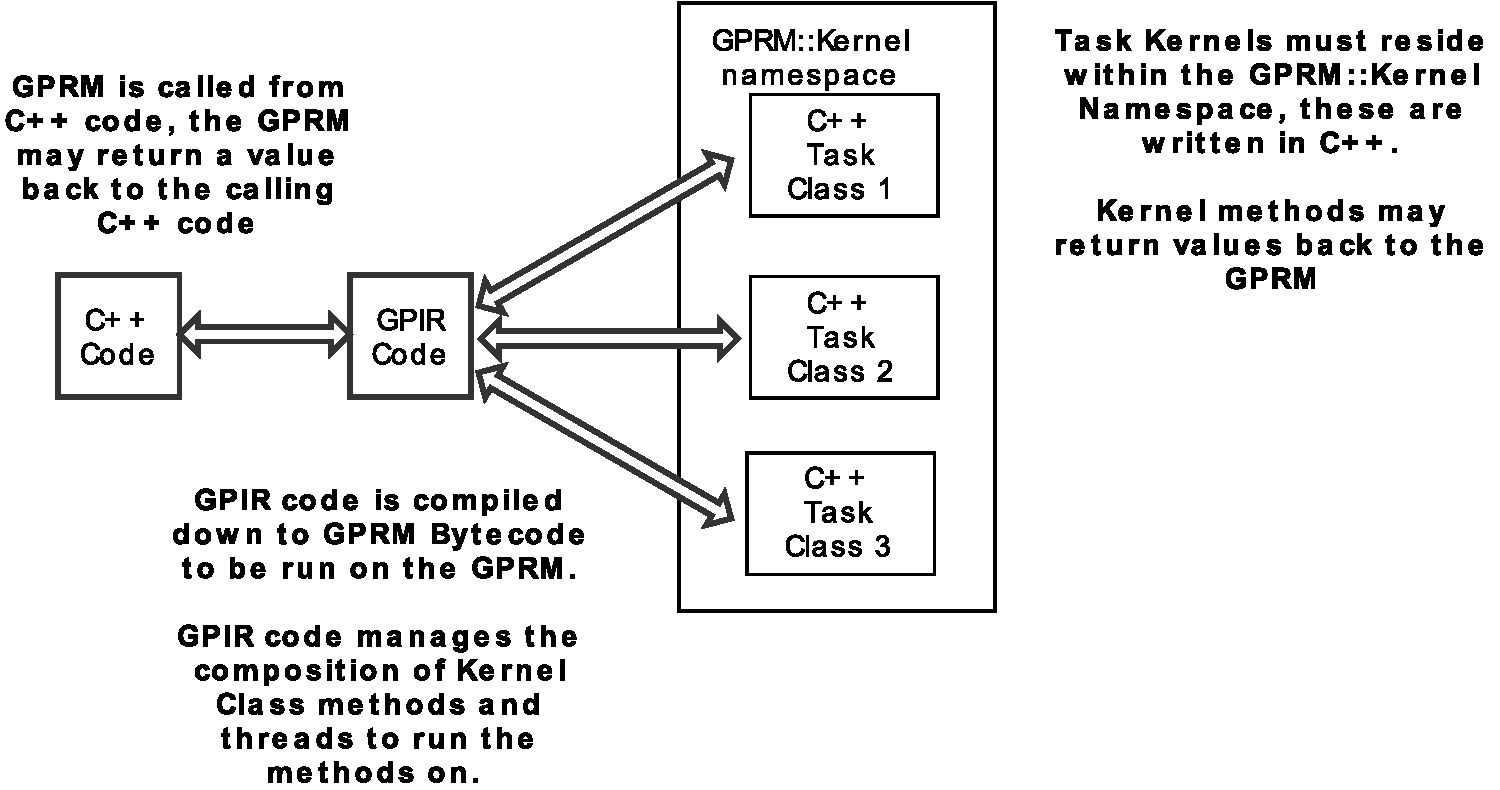
\includegraphics[width=\linewidth,height=\textheight,keepaspectratio]{../graphs/gprm.pdf}
}

\frame{
    \frametitle{GPIR}
    \begin{itemize}
        \item Glasgow Parallel Intermediate Representation language
        \item Purely functional S-expression like language like lisp or scheme.
        \item Evaluated in parallel by default with optional sequential evaluation
        \item Controls the composition of tasks.
    \end{itemize}
}

\frame{
    \frametitle{Problems with GPIR}
    \begin{itemize}
        \item Language isn't "consistent"  with the rest of the framework.
        \item Requires programmers to learn multiple languages which are vastly different.
        \item Still requires programmers to manually enter threads for each individual
              task to run on
    \end{itemize}
}

\section{GPC}

\subsection{GPC Language}
\frame{
    \frametitle{GPC}
    \begin{itemize}
        \item GPC (Glasgow Parallel C). Near subset of C++ with restrictions.
        \item Layer ontop of GPIR, can take advantage of parallel evaluation semantics
              of GPIR.
        \item Introduces two new keywords "seq" and "par" to denote sequential
              or parallel evaluation of code blocks.
    \end{itemize}
}

\frame{
    \frametitle{GPC Features}
    \begin{itemize}
        \item Purely functional, no multiple assignments
        \item Support for C++ objects, basic arithmetic operations, functions,
              types, restricted for-loops.
        \item Serial semantics.
        \item Jumping to labels is an expensive operation in the GPIR so
              inlining as much as possible to the point that  execution path can be determined at 
              compile time is useful.              
        \item However kernel calls for C++ can return values, for a turing complete
              language this is essentially the halting problem.
    \end{itemize}
}

\frame{
    \frametitle{Kernel type system}
    \begin{itemize}
        \item Resulting return values from calls to C++ Kernel Object methods 
              placed in the \texttt{GPRM::Kernel} namespace.
        \item Kernel types can be passed into kernel calls, but not 
              used as "GPRM" types, this prevents them being used
              for conditional statements, caught by type checker.
        \item Essentially keeps GPC purely functional while the "side effect"
              code is restricted to the kernels.
   \end{itemize}
}

\frame{
    \frametitle{Benefits of being a C++ subset}
    \begin{itemize}
        \item Being a subset of C++, we can define \texttt{seq} and \texttt{par}
              as no-ops, compiler ignores preprocessor directives. 
        \item Can be compiled using a C++ compiler, due to serial semantics
              behaviour should be the same as parallel version.
        \item Can use already available C++ tools to test.
    \end{itemize}
}

\section{Implementation}
    \frame{
            \frametitle{GPC Implementation}    
            \begin{itemize}
                \item Language compiler is implemented in Haskell
                \item Uses parsec library to parse/lex source
                \item Type and Scope checking then run over the AST
                \item Then interprets the AST to generate GPIR code
            \end{itemize}
}

\frame{
        \frametitle{Interpreter}
        \begin{itemize}
            \item Runs over AST
            \item Assigns threads to tasks
            \item Performs branch elimination on if statements. 
            \item Constant propogation and partial evaluation of expressions
            \item Function inlining for speed and for loop unrolling 
            \item Generates GPIR AST, can be "pretty printed" to GPIR source
        \end{itemize}
}


\raggedright

\frame{
    \frametitle{MergeSort Example}
    \lstinputlisting[style=myGPC]{GPRM_MergeSort.gpc}
}


\frame{
    \frametitle{MergeSort Example}
    \lstinputlisting[style=myGPIR]{GPRM_MergeSort.td}
}


\frame{
    \frametitle{Summary}
    \begin{itemize}
        \item Designed a purely functional language which is familiar to programmers
              which describes the composition of serial C++ tasks to be run in parallel
        \item Built the compiler for this language.
        \item Questions?    
    \end{itemize}
}



\end{document}




